\documentclass[11pt]{article}
\ProvidesPackage{calcpractices}[2026/05/14 AP Calculus BC shared preamble]
\usepackage[margin=1in]{geometry}
\usepackage{fancyhdr}
\usepackage{amsmath}
\usepackage{tikz}
\usepackage{pgfplots}
\usepackage{multicol}
\pgfplotsset{compat=1.18}

\pagestyle{fancy}
\fancyhf{}
\fancyhead[L]{AP Calculus BC}
\fancyhead[R]{Practice}
\fancyfoot[C]{\thepage}

\newcommand{\emptygraph}{
    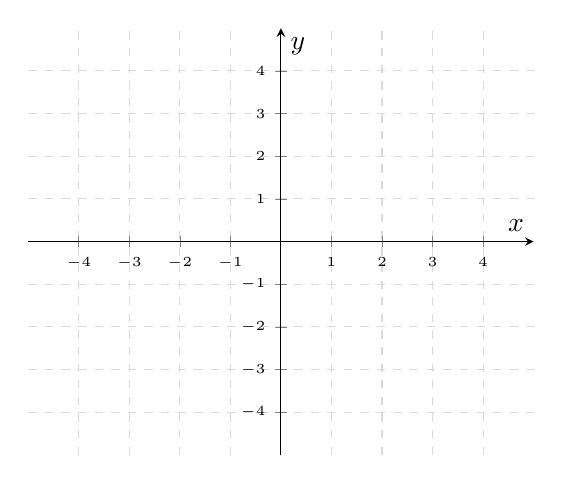
\begin{tikzpicture}
        \begin{axis}[
            axis lines = middle,
            grid = both,
            width=8cm,
            height=7cm,
            xmin=-5, xmax=5,
            ymin=-5, ymax=5,
            xtick={-4,-3,...,4},
            ytick={-4,-3,...,4},
            xlabel={$x$},
            ylabel={$y$},
            tick label style={font=\tiny},
            grid style={dashed, gray!30}
        ]
        \end{axis}
    \end{tikzpicture}
}

\newcommand{\smallgraph}{
    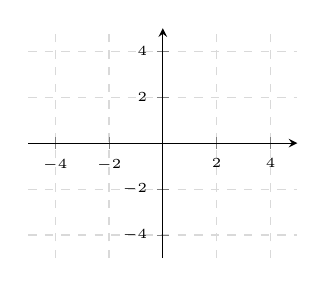
\begin{tikzpicture}
        \begin{axis}[
            axis lines = middle,
            grid = both,
            width=5cm,
            height=4.5cm,
            xmin=-5, xmax=5,
            ymin=-5, ymax=5,
            xtick={-4,-2,0,2,4},
            ytick={-4,-2,0,2,4},
            tick label style={font=\tiny},
            grid style={dashed, gray!30}
        ]
        \end{axis}
    \end{tikzpicture}
}

\fancyhead[C]{1.6 Trigonometric Functions}

\begin{document}

    \begin{enumerate}

        \item Given a circle with a central angle of $\dfrac{5\pi}{8}$ and a radius of 2 inches, find the arc length.

        \vspace{20ex}

        \item Given a circle with a radius of 2 mm and an arc length of $\dfrac{3\pi}{2}$ mm, find the central angle.

        \vspace{20ex}

        \noindent Determine if the function is even or odd.

        \begin{multicols}{2}
            \item secant\\[4ex]
            \item cotangent\\[4ex]
        \end{multicols}

        \item Find all of the trig values of $\theta$ if $\displaystyle \cos\theta = \dfrac{-15}{17}$, $\sin\theta > 0$.

        \vspace{33ex}

        \item Graph $\displaystyle y = 3\csc(3x + \pi) - 2$ and determine the period, amplitude, domain, range, and shifts.

        \emptygraph

        \newpage

        \item Graph $\displaystyle y = -4\tan\!\left(2x + \dfrac{\pi}{4}\right) + 1$ and determine the period, amplitude, domain, range, and shifts.

        \emptygraph

        \vspace{1ex}

        \item Graph $\displaystyle y = -\cos(3x - \pi) - 2$ and determine the period, amplitude, domain, range, and shifts.

        \emptygraph

        \newpage

        \item The table below shows average monthly temperatures for St.\ Louis for one year. Use the equation $\displaystyle y = a\sin(b(t-h)) + k$, where $y$ is in degrees F and $t$ is in months. Find the $b$-value (assume the period is 12 months), the amplitude $a$, the $k$ value, and the $h$ value. Write an equation and then superimpose it over a scatter plot of the data.\\[2ex]

        \noindent\begin{minipage}[t]{0.30\linewidth}
            \vspace{0pt}
            {\renewcommand{\arraystretch}{1.2}
                \begin{tabular}{|c|c|}
                    \hline
                    \multicolumn{2}{|c|}{\textbf{St.\ Louis Temps}} \\ \hline
                    \textbf{Month} & \textbf{Temp (${}^\circ$F)}    \\ \hline
                    1              & 34                             \\ \hline
                    2              & 30                             \\ \hline
                    3              & 39                             \\ \hline
                    4              & 44                             \\ \hline
                    5              & 58                             \\ \hline
                    6              & 67                             \\ \hline
                    7              & 78                             \\ \hline
                    8              & 80                             \\ \hline
                    9              & 72                             \\ \hline
                    10             & 63                             \\ \hline
                    11             & 51                             \\ \hline
                    12             & 40                             \\ \hline
                \end{tabular}}
        \end{minipage}\hfill%
        \begin{minipage}[t]{0.66\linewidth}
            \vspace{0pt}
            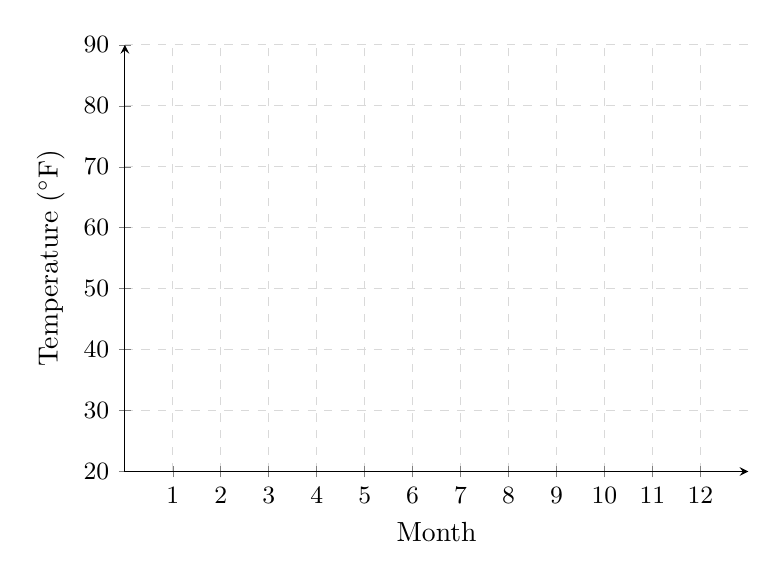
\begin{tikzpicture}
                \begin{axis}[
                        axis lines=left,
                        grid=both,
                        width=9.5cm, height=7cm,
                        xmin=0, xmax=13,
                        ymin=20, ymax=90,
                        xtick={1,2,...,12},
                        ytick={20,30,...,90},
                        xlabel={Month},
                        ylabel={Temperature (${}^\circ$F)},
                        tick label style={font=\small},
                        grid style={dashed, gray!30}]
                \end{axis}
            \end{tikzpicture}
        \end{minipage}

        \newpage

        \noindent Show that the function is one-to-one and graph its inverse.

        \begin{multicols}{2}
            \item $\displaystyle y = \cos x,\quad 0 \le x \le \pi$\\[1ex]\smallgraph
            \item $\displaystyle y = \tan x,\quad -\dfrac{\pi}{2} < x < \dfrac{\pi}{2}$\\[1ex]\smallgraph
        \end{multicols}

        \vspace{1ex}

        \noindent Give the measure of the angle in radians and degrees.

        \begin{multicols}{3}
            \item $\displaystyle \sin^{-1}(-0.5)$\\[5ex]
            \item $\displaystyle \cos^{-1}\!\left(\dfrac{\sqrt{2}}{2}\right)$\\[5ex]
            \item $\displaystyle \arctan\!\left(\dfrac{-\sqrt{3}}{3}\right)$\\[5ex]
        \end{multicols}

        \noindent Solve the equation in the specified interval.

        \begin{multicols}{2}
            \item $\displaystyle \csc x = 2,\quad 0 < x < 2\pi$\\[5ex]
            \item $\displaystyle \cot x = -1,\quad -\infty < x < \infty$\\[5ex]
        \end{multicols}

        \noindent Use the given information to find the values of the six trig functions at the angle $\theta$.

        \begin{multicols}{2}
            \item $\displaystyle \theta = \sin^{-1}\!\left(\dfrac{8}{17}\right)$\\[6ex]
            \item $\displaystyle \theta = \tan^{-1}\!\left(\dfrac{-5}{12}\right)$\\[6ex]
        \end{multicols}

        \item The point $\displaystyle P(-3, 4)$ is on the terminal side of $\theta$. Find the values of the six trig functions at $\theta$.

        \vspace{26ex}

        \noindent Evaluate the expression.

        \begin{multicols}{2}
            \item $\displaystyle \sin\!\left(\cos^{-1}\!\left(\dfrac{7}{11}\right)\right)$\\[5ex]
            \item $\displaystyle \tan\!\left(\sin^{-1}\!\left(\dfrac{9}{13}\right)\right)$\\[5ex]
        \end{multicols}

        \item The temperature in Fairbanks, Alaska is modeled by the graph below. Find the amplitude, period, horizontal shift, and vertical shift. Write two equations for the model, one with sine and one with cosine.\\[1ex]

        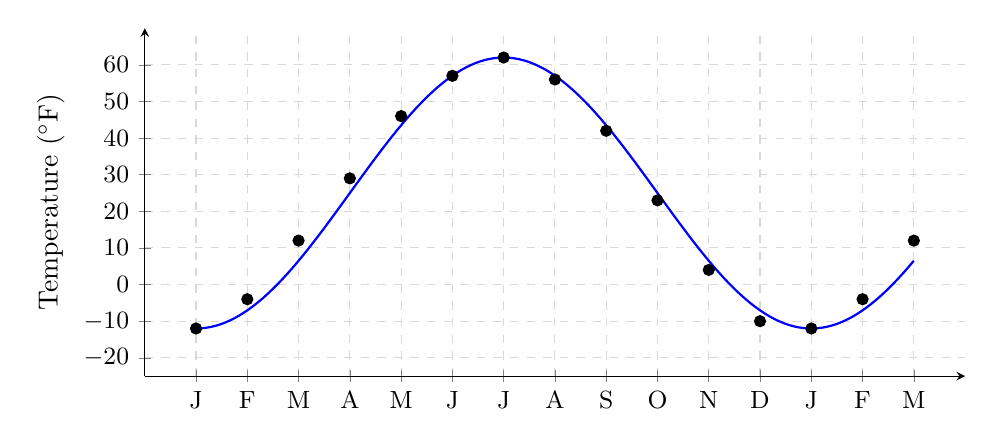
\begin{tikzpicture}
            \begin{axis}[
                    axis lines=left,
                    grid=both,
                    width=12cm, height=6cm,
                    xmin=0, xmax=16,
                    ymin=-25, ymax=70,
                    xtick={1,2,...,15},
                    xticklabels={J,F,M,A,M,J,J,A,S,O,N,D,J,F,M},
                    ytick={-20,-10,...,60},
                    ylabel={Temperature (${}^\circ$F)},
                    tick label style={font=\small},
                    grid style={dashed, gray!30}]
                \addplot[blue, thick, domain=1:15, samples=150]{37*sin(30*(x-4))+25};
                \addplot[only marks, mark=*, mark size=2pt, black] coordinates {
                        (1,-12)(2,-4)(3,12)(4,29)(5,46)(6,57)(7,62)(8,56)(9,42)(10,23)(11,4)(12,-10)
                        (13,-12)(14,-4)(15,12)};
            \end{axis}
        \end{tikzpicture}

    \end{enumerate}

\end{document}
